\documentclass{anstrans}
%%%%%%%%%%%%%%%%%%%%%%%%%%%%%%%%%%%
\title{Full-core multiphysics analysis of Molten Salt Reactor Experiment using parallel code}

\author{Andrei Rykhlevskii}

\email{andreir2@illinois.edu}

%%%% packages and definitions (optional)
\usepackage{graphicx} % allows inclusion of graphics
\usepackage{caption}  % allows center figures caption
\usepackage{booktabs} % nice rules (thick lines) for tables
\usepackage{microtype} % improves typography for PDF
\usepackage[section]{placeins}
\usepackage[acronym,toc]{glossaries}  % acronyms inclusion

%\newacronym{<++>}{<++>}{<++>}
\newacronym[longplural={metric tons of heavy metal}]{MTHM}{MTHM}{metric ton of heavy metal}
\newacronym{ABM}{ABM}{agent-based modeling}
\newacronym{ACDIS}{ACDIS}{Program in Arms Control \& Domestic and International Security}
\newacronym{AHTR}{AHTR}{Advanced High Temperature Reactor}
\newacronym{ANDRA}{ANDRA}{Agence Nationale pour la gestion des D\'echets RAdioactifs, the French National Agency for Radioactive Waste Management}
\newacronym{ANL}{ANL}{Argonne National Laboratory}
\newacronym{API}{API}{application programming interface}
\newacronym{ARCH}{ARCH}{autoregressive conditional heteroskedastic}
\newacronym{ARE}{ARE}{Aircraft Reactor Experiment}
\newacronym{ARFC}{ARFC}{Advanced Reactors and Fuel Cycles}
\newacronym{ARMA}{ARMA}{autoregressive moving average}
\newacronym{ASME}{ASME}{American Society of Mechanical Engineers}
\newacronym{ATWS}{ATWS}{Anticipated Transient Without Scram}
\newacronym{BDBE}{BDBE}{Beyond Design Basis Event}
\newacronym{BIDS}{BIDS}{Berkeley Institute for Data Science}
\newacronym{BOL}{BOL}{Beginning-of-Life}
\newacronym{BSD}{BSD}{Berkeley Software Distribution}
\newacronym{CAFCA}{CAFCA}{Code for Advanced Fuel Cycles Assessment}
\newacronym{CASL}{CASL}{Consortium for Advanced Simulation of Light Water Reactors}
\newacronym{CDTN}{CDTN}{Centro de Desenvolvimento da Tecnologia Nuclear}
\newacronym{CEA}{CEA}{Commissariat \`a l'\'Energie Atomique et aux \'Energies Alternatives}
\newacronym{CFD}{CFD}{Computational Fluid Dynamics}
\newacronym{CG}{CG}{Continuous Galerkin}
\newacronym{CI}{CI}{continuous integration}
\newacronym{CNEN}{CNEN}{Comiss\~{a}o Nacional de Energia Nuclear}
\newacronym{CNERG}{CNERG}{Computational Nuclear Engineering Research Group}
\newacronym{COMSOL}{COMSOL}{COMmon SOLution}
\newacronym{COSI}{COSI}{Commelini-Sicard}
\newacronym{COTS}{COTS}{commercial, off-the-shelf}
\newacronym{CSNF}{CSNF}{commercial spent nuclear fuel}
\newacronym{CTAH}{CTAHs}{Coiled Tube Air Heaters}
\newacronym{CUBIT}{CUBIT}{CUBIT Geometry and Mesh Generation Toolkit}
\newacronym{CURIE}{CURIE}{Centralized Used Fuel Resource for Information Exchange}
\newacronym{DAG}{DAG}{directed acyclic graph}
\newacronym{DANESS}{DANESS}{Dynamic Analysis of Nuclear Energy System Strategies}
\newacronym{DBE}{DBE}{Design Basis Event}
\newacronym{DESAE}{DESAE}{Dynamic Analysis of Nuclear Energy Systems Strategies}
\newacronym{DG}{DG}{Discontinuous Galerkin}
\newacronym{DHS}{DHS}{Department of Homeland Security}
\newacronym{DOE}{DOE}{Department of Energy}
\newacronym{DRACS}{DRACS}{Direct Reactor Auxiliary Cooling System}
\newacronym{DRE}{DRE}{dynamic resource exchange}
\newacronym{DSNF}{DSNF}{DOE spent nuclear fuel}
\newacronym{DYMOND}{DYMOND}{Dynamic Model of Nuclear Development }
\newacronym{EBS}{EBS}{Engineered Barrier System}
\newacronym{EDZ}{EDZ}{Excavation Disturbed Zone}
\newacronym{EIA}{EIA}{U.S. Energy Information Administration}
\newacronym{EPA}{EPA}{Environmental Protection Agency}
\newacronym{EP}{EP}{Engineering Physics}
\newacronym{FCO}{FCO}{Fuel Cycle Options}
\newacronym{FCT}{FCT}{Fuel Cycle Technology}
\newacronym{FEHM}{FEHM}{Finite Element Heat and Mass Transfer}
\newacronym{FEPs}{FEPs}{Features, Events, and Processes}
\newacronym{FHR}{FHR}{Fluoride-Salt-Cooled High-Temperature Reactor}
\newacronym{FLiBe}{FLiBe}{Fluoride-Lithium-Beryllium}
\newacronym{GCAM}{GCAM}{Global Change Assessment Model}
\newacronym{GDSE}{GDSE}{Generic Disposal System Environment}
\newacronym{GDSM}{GDSM}{Generic Disposal System Model}
\newacronym{GENIUSv1}{GENIUSv1}{Global Evaluation of Nuclear Infrastructure Utilization Scenarios, Version 1}
\newacronym{GENIUSv2}{GENIUSv2}{Global Evaluation of Nuclear Infrastructure Utilization Scenarios, Version 2}
\newacronym{GENIUS}{GENIUS}{Global Evaluation of Nuclear Infrastructure Utilization Scenarios}
\newacronym{GPAM}{GPAM}{Generic Performance Assessment Model}
\newacronym{GRSAC}{GRSAC}{Graphite Reactor Severe Accident Code}
\newacronym{GUI}{GUI}{graphical user interface}
\newacronym{HLW}{HLW}{high level waste}
\newacronym{HPC}{HPC}{high-performance computing}
\newacronym{HTC}{HTC}{high-throughput computing}
\newacronym{HTGR}{HTGR}{High Temperature Gas-Cooled Reactor}
\newacronym{IAEA}{IAEA}{International Atomic Energy Agency}
\newacronym{IEMA}{IEMA}{Illinois Emergency Mangament Agency}
\newacronym{INL}{INL}{Idaho National Laboratory}
\newacronym{IPRR1}{IRP-R1}{Instituto de Pesquisas Radioativas Reator 1}
\newacronym{IRP}{IRP}{Integrated Research Project}
\newacronym{ISFSI}{ISFSI}{Independent Spent Fuel Storage Installation}
\newacronym{ISRG}{ISRG}{Independent Student Research Group}
\newacronym{JFNK}{JFNK}{Jacobian-Free Newton Krylov}
\newacronym{LANL}{LANL}{Los Alamos National Laboratory}
\newacronym{LBNL}{LBNL}{Lawrence Berkeley National Laboratory}
\newacronym{LCOE}{LCOE}{levelized cost of electricity}
\newacronym{LDRD}{LDRD}{laboratory directed research and development}
\newacronym{LFR}{LFR}{Lead-Cooled Fast Reactor}
\newacronym{LGPL}{LGPL}{Lesser GNU Public License}
\newacronym{LLNL}{LLNL}{Lawrence Livermore National Laboratory}
\newacronym{LMFBR}{LMFBR}{Liquid-Metal-cooled Fast Breeder Reactor}
\newacronym{LOFC}{LOFC}{Loss of Forced Cooling}
\newacronym{LOHS}{LOHS}{Loss of Heat Sink}
\newacronym{LOLA}{LOLA}{Loss of Large Area}
\newacronym{LP}{LP}{linear program}
\newacronym{LWR}{LWR}{Light Water Reactor}
\newacronym{MARKAL}{MARKAL}{MARKet and ALlocation}
\newacronym{MA}{MA}{minor actinide}
\newacronym{MCNP}{MCNP}{Monte Carlo N-Particle code}
\newacronym{MILP}{MILP}{mixed-integer linear program}
\newacronym{MIT}{MIT}{the Massachusetts Institute of Technology}
\newacronym{MOAB}{MOAB}{Mesh-Oriented datABase}
\newacronym{MOOSE}{MOOSE}{Multiphysics Object-Oriented Simulation Environment}
\newacronym{MOX}{MOX}{mixed oxide}
\newacronym{MPI}{MPI}{Message Passing Interface}
\newacronym{MSBR}{MSBR}{Molten Salt Breeder Reactor}
\newacronym{MSFR}{MSFR}{Molten Salt Fast Reactor}
\newacronym{MSRE}{MSRE}{Molten Salt Reactor Experiment}
\newacronym{MSR}{MSR}{Molten Salt Reactor}
\newacronym{NAGRA}{NAGRA}{National Cooperative for the Disposal of Radioactive Waste}
\newacronym{NCSA}{NCSA}{National Center for Supercomputing Applications}
\newacronym{NEAMS}{NEAMS}{Nuclear Engineering Advanced Modeling and Simulation}
\newacronym{NEUP}{NEUP}{Nuclear Energy University Programs}
\newacronym{NFCSim}{NFCSim}{Nuclear Fuel Cycle Simulator}
\newacronym{NFC}{NFC}{Nuclear Fuel Cycle}
\newacronym{NGNP}{NGNP}{Next Generation Nuclear Plant}
\newacronym{NMWPC}{NMWPC}{Nuclear MW Per Capita}
\newacronym{NNSA}{NNSA}{National Nuclear Security Administration}
\newacronym{NPRE}{NPRE}{Department of Nuclear, Plasma, and Radiological Engineering}
\newacronym{NQA1}{NQA-1}{Nuclear Quality Assurance - 1}
\newacronym{NRC}{NRC}{Nuclear Regulatory Commission}
\newacronym{NSF}{NSF}{National Science Foundation}
\newacronym{NSSC}{NSSC}{Nuclear Science and Security Consortium}
\newacronym{NUWASTE}{NUWASTE}{Nuclear Waste Assessment System for Technical Evaluation}
\newacronym{NWF}{NWF}{Nuclear Waste Fund}
\newacronym{NWTRB}{NWTRB}{Nuclear Waste Technical Review Board}
\newacronym{OCRWM}{OCRWM}{Office of Civilian Radioactive Waste Management}
\newacronym{ORION}{ORION}{ORION}
\newacronym{ORNL}{ORNL}{Oak Ridge National Laboratory}
\newacronym{PARCS}{PARCS}{Purdue Advanced Reactor Core Simulator}
\newacronym{PBAHTR}{PB-AHTR}{Pebble Bed Advanced High Temperature Reactor}
\newacronym{PBFHR}{PB-FHR}{Pebble-Bed Fluoride-Salt-Cooled High-Temperature Reactor}
\newacronym{PEI}{PEI}{Peak Environmental Impact}
\newacronym{PH}{PRONGHORN}{PRONGHORN}
\newacronym{PRKE}{PRKE}{Point Reactor Kinetics Equations}
\newacronym{PSPG}{PSPG}{Pressure-Stabilizing/Petrov-Galerkin}
\newacronym{PWAR}{PWAR}{Pratt and Whitney Aircraft Reactor}
\newacronym{PWR}{PWR}{Pressurized Water Reactor}
\newacronym{PetSc}{PetSc}{Portable, Extensible Toolkit for Scientific Computation}
\newacronym{PyNE}{PyNE}{Python toolkit for Nuclear Engineering}
\newacronym{PyRK}{PyRK}{Python for Reactor Kinetics}
\newacronym{QA}{QA}{quality assurance}
\newacronym{RDD}{RD\&D}{Research Development and Demonstration}
\newacronym{RD}{R\&D}{Research and Development}
\newacronym{RELAP}{RELAP}{Reactor Excursion and Leak Analysis Program}
\newacronym{RIA}{RIA}{Reactivity Insertion Accident}
\newacronym{RIF}{RIF}{Region-Institution-Facility}
\newacronym{SFR}{SFR}{Sodium-Cooled Fast Reactor}
\newacronym{SINDAG}{SINDA{\textbackslash}G}{Systems Improved Numerical Differencing Analyzer $\backslash$ Gaski}
\newacronym{SKB}{SKB}{Svensk K\"{a}rnbr\"{a}nslehantering AB}
\newacronym{SNF}{SNF}{spent nuclear fuel}
\newacronym{SNL}{SNL}{Sandia National Laboratory}
\newacronym{STC}{STC}{specific temperature change}
\newacronym{SUPG}{SUPG}{Streamline-Upwind/Petrov-Galerkin}
\newacronym{SWF}{SWF}{Separations and Waste Forms}
\newacronym{SWU}{SWU}{Separative Work Unit}
\newacronym{TRIGA}{TRIGA}{Training Research Isotope General Atomic}
\newacronym{TRISO}{TRISO}{Tristructural Isotropic}
\newacronym{TSM}{TSM}{Total System Model}
\newacronym{TSPA}{TSPA}{Total System Performance Assessment for the Yucca Mountain License Application}
\newacronym{ThOX}{ThOX}{thorium oxide}
\newacronym{UFD}{UFD}{Used Fuel Disposition}
\newacronym{UML}{UML}{Unified Modeling Language}
\newacronym{UOX}{UOX}{uranium oxide}
\newacronym{UQ}{UQ}{uncertainty quantification}
\newacronym{US}{US}{United States}
\newacronym{UW}{UW}{University of Wisconsin}
\newacronym{VISION}{VISION}{the Verifiable Fuel Cycle Simulation Model}
\newacronym{VV}{V\&V}{verification and validation}
\newacronym{WIPP}{WIPP}{Waste Isolation Pilot Plant}
\newacronym{YMR}{YMR}{Yucca Mountain Repository Site}
\newacronym{gpm}{gpm}{gallons per minute}

\graphicspath{{figures/}}
\captionsetup{justification   = raggedright,
              singlelinecheck = false}
\newcommand{\SN}{S$_N$}
\renewcommand{\vec}[1]{\bm{#1}} %vector is bold italic
\newcommand{\vd}{\bm{\cdot}} % slightly bold vector dot
\newcommand{\grad}{\vec{\nabla}} % gradient
\newcommand{\ud}{\mathop{}\!\mathrm{d}} % upright derivative symbol
\makeglossaries

\begin{document}
%%%%%%%%%%%%%%%%%%%%%%%%%%%%%%%%%%%%%%%%%%%%%%%%%%%%%%%%%%%%%%%%%%%%%%%%%%%%%%%%
\section{Introduction}
The \gls{MSR} is an advanced type of reactor which was developed at \gls{ORNL} 
in the 1950s and was operated in the 1960s. In the MSR, fluorides of fissile 
and/or fertile materials (i.e. UF$_4$, PuF$_3$ and/or ThF$_4$) are mixed with 
carrier salts to form a liquid fuel which is circulated in a loop-type primary 
circuit \cite{haubenreich_experience_1970}. This innovation leads to immediate 
advantages over traditional, solid-fueled, reactors. These include 
near-atmospheric pressure in the primary loop, relatively high coolant 
temperature, outstanding neutron economy, a high level of inherent safety, 
reduced fuel preprocessing, and the ability to continuously remove fission 
products and add fissile and/or fertile elements \cite{leblanc_molten_2010}. 

%%%%%%%%%%%%%%%%%%%%%%%%%%%%%%%%%%%%%%%%%%%%%%%%%%%%%%%%%%%%%%%%%%%%%%%%%%%%%%%%
\section{LITERATURE REVIEW}
\gls{MSR} modeling efforts describe steady-state and
transient behavior. Krepel et al. extended the in-house \gls{LWR}
diffusion code DYN3D to consider drift of delayed neutron precursors alongside
the reactor temperature profile, re-casting the extended code as
DYN3D-MSR \cite{krepel_dyn3d-msr_2007}. That work compared DYN3D-MSR against
experimental \gls{MSRE} data and then used it to simulate local fuel channel
blockages as well as local temperature perturbations. In a similar vein, Kophazi
et. al. used iterative coupling between in-house three-dimensional neutronic and
one-dimensional heat conduction models DALTON and THERM to analyze normal 
\gls{MSRE} operation as well as channel-blocking-incident
transients \cite{kophazi_development_2009}. The Kophazi model added entrance 
effects of heat transfer coefficients as well as thermal
coupling between fuel channels through moderator heat conduction. More recently,
Cammi et. al. performed a 2D-axisymmetric single-channel analysis of the
\gls{MSBR} using the commercial finite element package COMSOL
Multiphysics \cite{cammi_multi-physics_2011}. That work directly solved the 
fuel salt velocity field, used heterogeneous group constants
in fuel and moderator regions, and employed a software package (COMSOL)
intrinsically designed for coupled multi-physics simulation.
Additionally, Aufiero et. al \cite{aufiero_development_2014} have begun to 
approach transient simulations in the \gls{MSFR} by directly coupling Serpent 2 
Monte Carlo neutronics with OpenFOAM \cite{weller_tensorial_1998} thermal-hydraulics.

\section{Approach and method}
Recently developed multiphysics code Moltres
\cite{lindsay_moltres_2017} could be employed for simulating \glspl{MSR}.  By implementing
deterministic neutronics and thermal hydraulics in the context of the
\gls{MOOSE} finite element modeling framework, Moltres solves arbitrary-group
neutron diffusion, temperature, and precursor governing equations in anywhere
from one to three dimensions and can be deployed on an arbitrary number of
processing units. Through its computing power, Moltres is devoted to previously
unmatched fidelity in coupled neutronics and thermal hydraulics \gls{MSR}
simulation.

Moreover, Moltres depends on the \gls{MOOSE} framework, \cite{gaston_physics-based_2015} which is \gls{LGPL} code that itself 
leans on LibMesh \cite{kirk_libmesh:_2006}, a \gls{LGPL} finite element library, and PetSc \cite{satish_balay_petsc_2015}, a
\gls{BSD}-licensed toolkit for solving nonlinear equations yielded by 
discretizing PDEs. \gls{MOOSE} and LibMesh translate weak PDE forms defined by applications (e.g. Moltres) into residual and Jacobian functions. These functions are the inputs into PetSc Newton-Raphson solution routines. All codes use MPI for parallel communication and are easily deployed on massively-parallel cluster-computing platforms. \gls{MOOSE} applications by
default use monolithic and implicit methods ideal for closely-coupled and multi-scale physics, such as the model problem described in this work. However, Moltres can also use explicit time-stepping routines as well as segregated solution methods, making it extensible to myriad future modeling challenges.

In Moltres, neutrons are described with time-dependent multi-group diffusion theory: 

\hspace*{-0.7cm} 
$\frac{1}{v_g}\frac{\partial \phi_g}{\partial t} - \nabla \cdot D_g
\nabla \phi_g + \Sigma_g^r \phi_g = 
\chi_g^p \sum_{g' = 1}^G (1 - \beta) \nu \Sigma_{g'}^f \phi_{g'} + $
\begin{equation}
\sum_{g \ne g'}^G \Sigma_{g'\rightarrow g}^s \phi_{g'}
+ \chi_g^d \sum_i^I \lambda_i C_i
\end{equation}

\hspace*{-0.7cm} 
$v_g = \mbox{speed of neutrons in group g} \\
        \phi_g = \mbox{flux of neutrons in group g} \\
        t = \mbox{time} \\
        D_g = \mbox{diffusion coefficient for neutrons in group g} \\
        \Sigma_g^r = \mbox{macro removal cross-section from group g} \\
        \Sigma_{g'\rightarrow g}^s = \mbox{macroscopic cross-section of
        scattering from g' to g} \\
        \chi_g^p = \mbox{prompt fission spectrum, neutrons in group g} \\
        G = \mbox{number of discrete groups, g} \\
        \nu = \mbox{number of neutrons produced per fission} \\
        \Sigma_g^f = \mbox{macro cross-section for fission in group g} \\
        \chi_g^d = \mbox{delayed fission spectrum, neutrons in group g} \\
        I = \mbox{number of delayed neutron precursor groups} \\
        \beta = \mbox{delayed neutron fraction}\\
        \lambda_i = \mbox{average decay constant of delayed neutron precursors in i} \\
        C_i = \mbox{concentration of delayed neutron precursors in group i}$

\vspace*{0.25cm} 
Delayed neutron precursors are described by equation:

\begin{align}
        \frac{\partial C_i}{\partial t} &= \sum_{g'= 1}^G \beta_i \nu
        \Sigma_{g'}^f \phi_{g'} - \lambda_i C_i - \frac{\partial}{\partial z} u
        C_i 
\end{align}

with the last term representing the effect of fuel advection. The governing
equation for the temperature is given by:

\begin{align}
        \rho_fc_{p,f}\frac{\partial T_f}{\partial t} &+ \nabla\cdot\left(\rho_f
        c_{p,f} \vec{u}\cdot T_f -k_f\nabla T_f\right) =  Q_f
\end{align}
  $\rho_f = \mbox{density of fuel salt}\\
  c_{p,f} = \mbox{specific heat capacity of fuel salt}\\
  T_f = \mbox{temperature of fuel salt}\\
  \vec{u} = \mbox{velocity of fuel salt}\\
  k_f = \mbox{thermal conductivity of fuel salt}\\
  Q_f = \mbox{source term}$


in the fuel, where the source term $Q_f$ is defined by:

\begin{equation}
  Q_f = \sum_{g=1}^G \epsilon_{f,g}\Sigma_{f,g}\phi_g
  \label{eq:fuel_source}
\end{equation}

In the moderator, the governing equation for temperature is given by:

\begin{align}
        \rho_gc_{p,g}\frac{\partial T_g}{\partial t} &+
        \nabla\cdot\left(-k_g\nabla T_g\right) =  Q_g
  \label{eq:moderator_temp}
\end{align}

Group constants must be generated by the modeler with either Serpent
\cite{leppanen_serpent_2015} or SCALE \cite{dehart_reactor_2011}. Moltres 
interpolates group constant temperature dependence from prepared tables, which must be
constructed separately for fuel and moderator regions. 

\begin{figure}[hbp!] % replace 't' with 'b' to 
  \centering
  \vspace{-0.3em}
  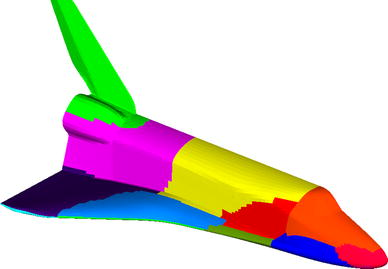
\includegraphics[width=0.95\linewidth]{fig3.jpg}
  \caption{Element-based domain decomposition of a surface mesh into 16 subdomains \cite{kirk2006}.}
  \vspace{-0.6em}
  \label{fig:decomp}
\end{figure}
\FloatBarrier

\section{Objectives}

In this study set of equations (1-5) in 2-D geometry (r-z) for well-studied \gls{MSRE} was solved using MOOSE-based multiphysics code Moltres and results were compared with reference \cite{briggs_molten-salt_1964}. Moltres predicted temperature profiles considered with cosinusoidal gamma heating for the hottest channel and adjacent graphite. It should be noted that the ORNL MSRE design calculations, conducted in 1963-1964, were 32-group calculations using legacy computing tools (GAM-I, MODRIC, and EQUIPOSE, and THERMOS). Those calculations were conducted in two-dimensional R-Z geometry (a cylinder with angular symmetry), with 20 spatial regions. 

Secondly, strong and weak scaling study was performed to find out appropriateness using Moltres for heavy computing full-core analysis and estimate "sweet" spot for large-scale calculations. Moreover, the results of scaling study clearly show the limitation of parallelization methods used in Moltres.

Finally, relative performance monolithic vs. segregated solution was considered. We usually use Moltres multiphysics code in the monolithic mode when it solves all equations in one element and after convergence switch to next element. To verify the relative efficiency of this approach finite-difference parallel solver for the simplified 2-D case was developed to solve one-group neutron diffusion equation for zero nuclear data and vacuum boundary conditions to estimate strong and weak scaling efficiency to compare with Moltres. For fair comparison (Moltres solves 5 equations while developed solver only 1) execution time for segregated solver was multiplied by 5.

\section{Parallelization}

MOOSE framework uses LibMesh finite element library to solve set of physics equations. Different 
finite element formulations may be applied including Galerkin, Petrov-Galerkin, and discontinuous
 Galerkin methods \cite{kirk2006}. Parallelism is achieved using domain decomposition through mesh partitioning,
 in which each processor contains the global mesh but in general computes only on a particular subset. 
 Parallel implicit linear systems are supported via an interface with the PETSc library. 

A standard non-overlapping domain decomposition approach is used in LibMesh to achieve data distribution 
on parallel computers as shown in Fig.~\ref{fig:decomp}. The elements in each subdomain are assigned to an individual processor. The two primary metrics in judging the quality of a partition are the subdomain mesh size and the number of "edge cuts" in the resulting partition. For a mesh composed of a single type of element, each subdomain should contain an equal number of elements so that the resulting domain decomposition is load balanced across all available processors. Usually, for \gls{MSR} simulation adaptive mesh refinement and coarsening (AMR/C) scheme provided by LibMesh is employed. AMR/C allows do not explicitly specify domain decomposition, and provides optimal parallel performance with minimal user's efforts.
 
Developed C++/MPI code has using finite-difference iterative method with a fixed number of iterations (>4000) to solve one-group neutron diffusion equation in a 2-D mesh. For simplicity 2-D Poisson's equation which is similar to one-group neutron diffusion equation was considered. At almost every grid point (i,j) the finite difference approximation to Poisson's equation is:
\begin{equation}
\frac{u_{i-1,j} - 2u_{i,j}+u_{i+1,j}}{h^2} + \frac{u_{i,j-1} - 2u_{i,j}+u_{i,j+1}}{h^2})
 = -f(x_i, y_j)
\end{equation}

Five-point stencil of the 2-D finite difference approximation shown in Fig.~\ref{fig:stencil}

\begin{figure}[thbp!] % replace 't' with 'b' to 
  \centering
  \vspace{-0.3em}
  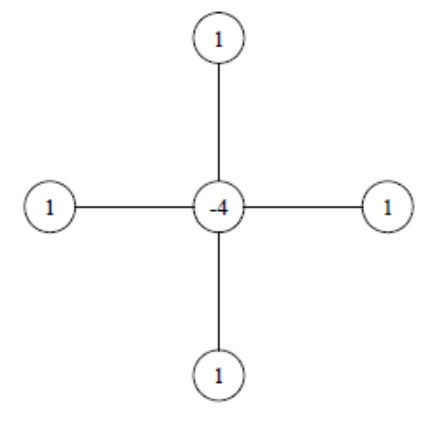
\includegraphics[width=0.75\linewidth]{stencil.png}
  \caption{5-point stencil for 2-D finite difference approximation.}
  \vspace{-0.6em}
  \label{fig:stencil}
\end{figure}
\FloatBarrier

Natural row-wise ordering is completely sequential, hence, reordering methods required. For Jacobi interative method best reordering strategy is red-black ordering when color the alternate grid points in each dimension red or black (Fig.~\ref{fig:stencil_red_black}). 

\begin{figure}[thbp!] % replace 't' with 'b' to 
  \centering
  \vspace{-0.3em}
  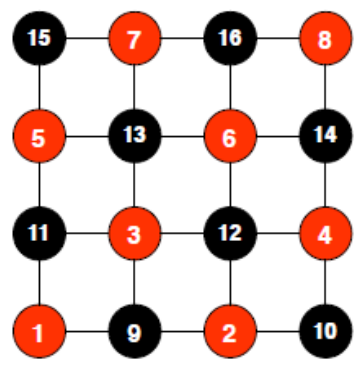
\includegraphics[width=0.75\linewidth]{red-black-ordering.png}
  \caption{Red-Black Ordering.}
  \vspace{-0.6em}
  \label{fig:stencil_red_black}
\end{figure}
\FloatBarrier

To implement selected reordering strategy first iterates on red grid point only:
\begin{equation}
u_{i,j}^{(k+1)} = (1-w)u_{i,j}^{(k)} + w/4 (h^2f_{i,j} + u_{i-1,j}^{(k)} + u_{i,j-1}^{(k)} + u_{i+1,j}^{(k)} + u_{i,j+1}^{(k)})
\end{equation}

Then iterates on black 	points only:
\begin{equation}
u_{i,j}^{(k+1)} = (1-w)u_{i,j}^{(k)} + w/4 (h^2f_{i,j} + u_{i-1,j}^{(k)} + u_{i,j-1}^{(k)} + u_{i+1,j}^{(k)} + u_{i,j+1}^{(k)})
\end{equation}
After that algorithm sends/receives values of the black-points at the boarder of the subdomain to neighboring processes and compute residual to check convergence (for scaling study number of iterations was fixed).

Preconditioned Conjugate Gradient (CG) method was used to accelerate convergence rate. Parallelization implemented using 2-D sub-matrices decomposition, when the 2D domain is divided into multiple sub-domains depending on the available number of computer nodes Fig.~\ref{fig:parallel} For interior points, neutron diffusion equation will be solved implicitly by Jacobi iterative scheme in combining with the boundary conditions. At the interface points of interior subdomains, the equation will be solved by explicit iterative schemes. The proposed approach fulfills the suitability for the implementation on Linux PC cluster through the minimization of inter-process communication by restricting the exchange of data to the interface between the sub-domains. To examine the efficiency and accuracy of the iterative algorithm, several numerical experiments using different number of nodes of the Linux PC cluster was conducted. The performance metrics should clearly show the benefit of using multicore system in terms of execution time reduction and speedup with respect to the sequential running in a single core.
\begin{figure}[thbp!] % replace 't' with 'b' to 
  \centering
  \vspace{-0.3em}
  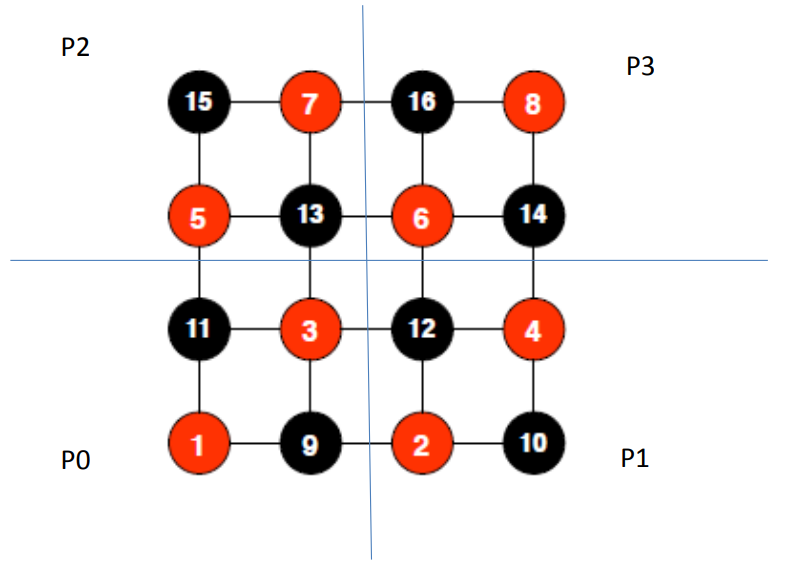
\includegraphics[width=0.95\linewidth]{parallel.png}
  \caption{Red-Black Ordering parallelization.}
  \vspace{-0.6em}
  \label{fig:parallel}
\end{figure}
\FloatBarrier

\section{Results}
\subsection{Comparison with \gls{MSRE}}

Fig.~\ref{fig:temp_compare} shows a comparison between Moltres predicted temperature and \gls{MSRE} design calculations
\cite{briggs_molten-salt_1964} in the hottest channel and adjacent graphite.

The profile shapes are in decent qualitative agreement with both Moltres and
\gls{MSRE} calculations showing a peak in graphite temperature before the
reactor outlet. Fuel temperature increases monotonically in both Moltres and
\gls{MSRE} models. In the \gls{MSRE} design, the moderator
temperature at the reactor inlet is about 11 K larger than the
fuel temperature, whereas the temperatures are about the same in the Moltres
model. This difference is likely because the \gls{MSRE} design model
neglected axial heat conduction \cite[p. 99]{briggs_molten-salt_1964}.

\begin{figure}[htpb]
    \centering
    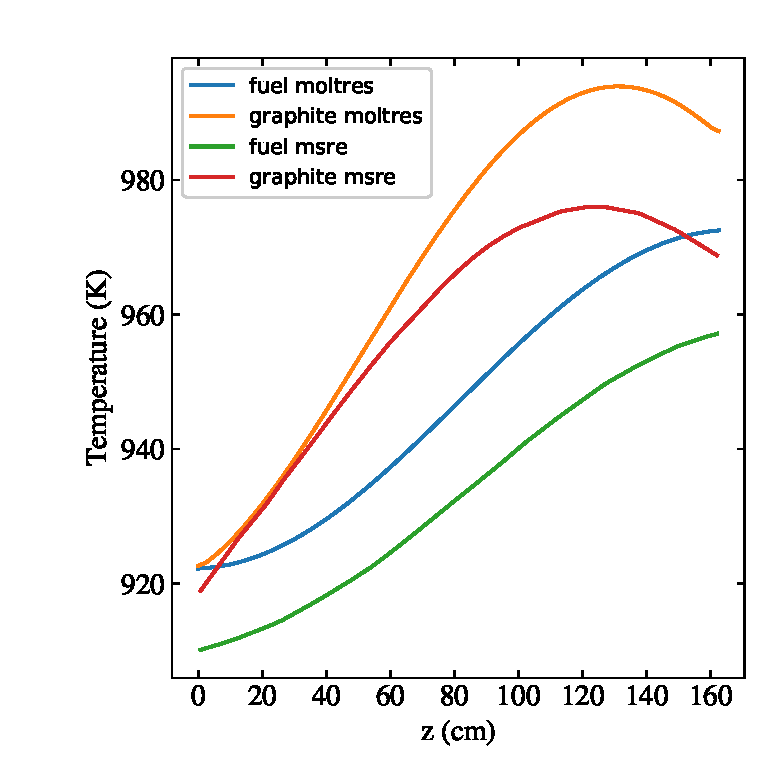
\includegraphics[width=\linewidth]{combined_msre_moltres_axial_temps.eps}
    \caption{Moltres and \gls{MSRE} design
      \cite[p. 99]{briggs_molten-salt_1964} predicted axial temperature profiles in hottest channel
      and adjacent graphite}
    \label{fig:temp_compare}
\end{figure}

Fig.~\ref{fig:radial_fluxes_compare} compares the fast and thermal neutron fluxes at
the reactor mid-plane ($z=H/2$) for Moltres and \gls{MSRE} design models. Local
thermal flux growth and fast flux decay in moderator regions and visa versa in
fuel regions are apparent in the Moltres calculation. The Moltres flux
magnitudes are in good agreement with the magnitudes from the \gls{MSRE} design
calculations \cite[p. 92]{briggs_molten-salt_1964}. The peak fast to thermal
flux ratio is approximately 3.5 in the \gls{MSRE} design calculation as opposed
to a ratio of 3 for the Moltres calculation. Control rod thimbles and an extra
volume of surrounding fuel not included in the Moltres calculations cause the
depression in the thermal flux in the \gls{MSRE} profile.

\begin{figure}[htpb]
    \centering
      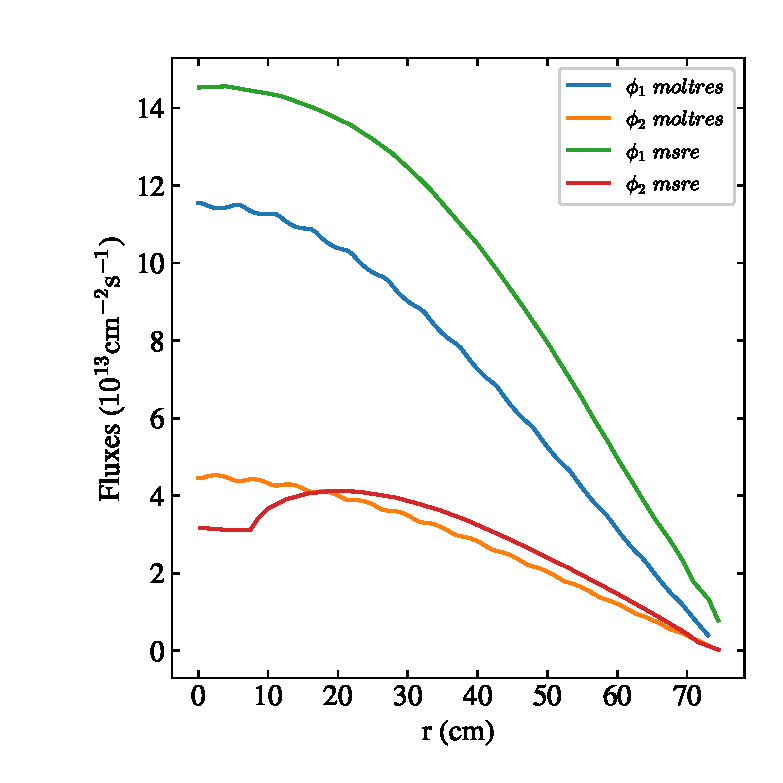
\includegraphics[width=\linewidth]{combined_msre_moltres_radial.eps}
      \caption{The thermal and fast flux profiles at the core mid-plane
        ($z=H/2$) for the Moltres 2-D cylindrical axisymmetric model and the
        \gls{MSRE} design model \cite[p. 92]{briggs_molten-salt_1964} ($r=0$ is
        radial center of core).}
    \label{fig:radial_fluxes_compare}
\end{figure}

Fig.~\ref{fig:axial_fluxes_compare} compares the axial flux profiles calculated by
Moltres and the \gls{ORNL} \gls{MSRE} design model. The radii for the plots are
chosen to correspond to the peak of the thermal flux in both cases; for the
\gls{ORNL} calculations this is 21.336 cm (8.4 inches) from the core center-line because of
the effect of the control rod thimbles and extra fuel along the
center-line. Once again, the plots are in decent agreement. The \gls{ORNL}
calculations include the lower and upper plena which are not included in this
report's Moltres model. Consequently, the \gls{MSRE} lines extend to lower and
higher z-values than the Moltres lines. Additionally, absorption
in the plena cause deviation of the thermal flux from a sinusoidal shape in the
\gls{MSRE} design case. The peak power density from the \gls{MSRE} calculation
is 31 kW/L; the corresponding value for Moltres is 29 kW/L.

\begin{figure}[htpb]
    \centering
    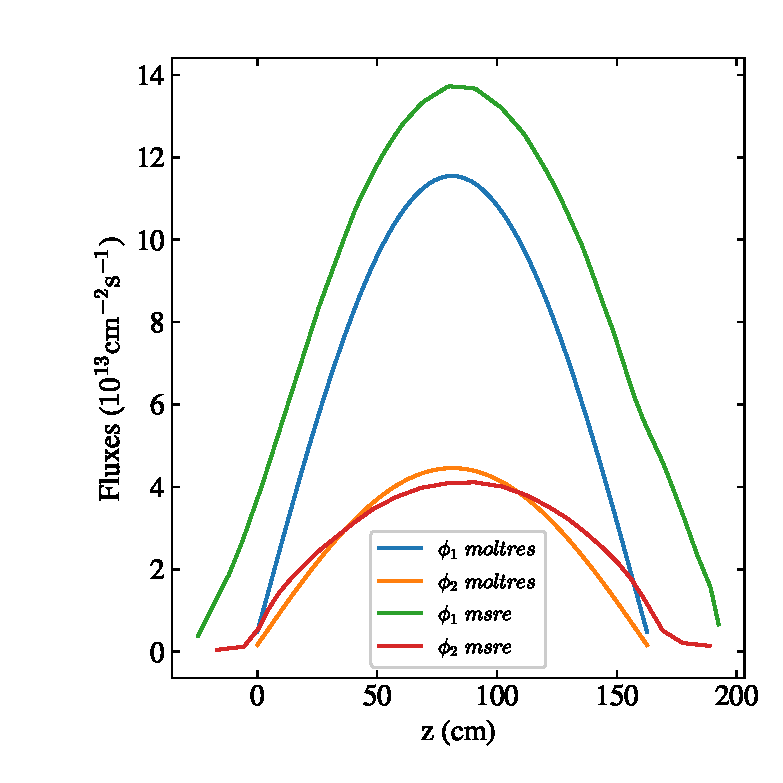
\includegraphics[width=\linewidth]{combined_msre_moltres_axial.eps}
    \caption{Moltres axial flux profiles along the core center line and \gls{MSRE}
    design axial flux profiles 21.336 cm (8.4 inches) from the core center line \cite[p. 91]{briggs_molten-salt_1964}.}
    \label{fig:axial_fluxes_compare}
\end{figure}

\subsection{Moltres scaling study}
Parallelization in Moltres is implemented via LibMesh, which includes a set of
utilities for massively parallel finite element based computations, including
mesh input/output, a finite element library, and an interface for connections with
solver packages. Employing LibMesh provides Moltres with
significant flexibility including the ability to swap out solver libraries
such as PetSc, which includes an expanding suite of parallel linear and
nonlinear solvers. Problem domain decomposition relies on LibMesh mesh
adaptation capabilities for running on a specific number of processors and
can either be performed manually before the start of the simulation or
automatically at the parameters of computation.

We conducted strong and weak scaling studies to characterize parallel
performance in Moltres.
In case of strong scaling, the problem size remains fixed but the number of
processors is increased. Strong scaling studies seek to identify an
optimal ratio between the number of processors and elements for the most
rapid and power-efficient computation for a given problem. We measured
Moltres strong scaling with a simple 2D axisymmetric
case for various problem sizes separately for intra-node (2,820; 5,640;
11,280 and 28,200 elements) and extra-node (86,655; 173,310; 317,735;
664,355 elements) setup on Blue Waters' XK7 nodes (two AMD 6276 Interlagos
CPU per node, 16 floating-point bulldozer core units per node or 32 "integer"
cores per node, nominal clock speed is 2.45 GHz).

Fig.~\ref{fig:intra_strong_scaling} shows the simulation speed in seconds
per element vs. the number of cores on 1 node (maximum 32 cores). Up to 8
cores, larger problems required considerably more time per
element because of cache overhead. However, beyond 8 cores, scaling demonstrates
asymptotic dependence on the number of processors due to increasing
communication costs. The best parallel efficiency for the intra-node study
is approximately 89\% and has been achieved for the largest problem
(28,200 elements).

\begin{figure}[htpb!]
  \centering
  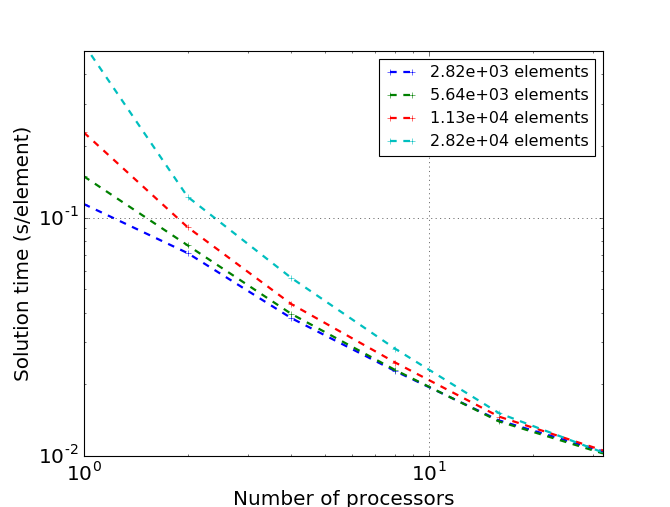
\includegraphics[width=\linewidth]{intra-node_strong.png}
  \caption{Moltres intra-node strong scaling efficiency for various problem
        sizes, for $n_{cores} \in [1,32]$.}
  \label{fig:intra_strong_scaling}
\end{figure}

Fig.~\ref{fig:extra_strong_scaling} shows Moltres strong scaling up to 768
processors. This takes into account communication costs between nodes.
Similar to the intra-node study, when fewer than 128 cores were used,
cache overhead causes performance slow down for larger problems. However,
beyond 256 cores, the simulation time per element remains almost constant
for small cases (86,655 and 173,310 elements) and slighly decreases for the
two larger problems. For extra-node scaling, parallel efficiency also grows
with the problem size and reaches an optimal value of 73\% for 664,355 elements.

\begin{figure}[htpb]
  \centering
  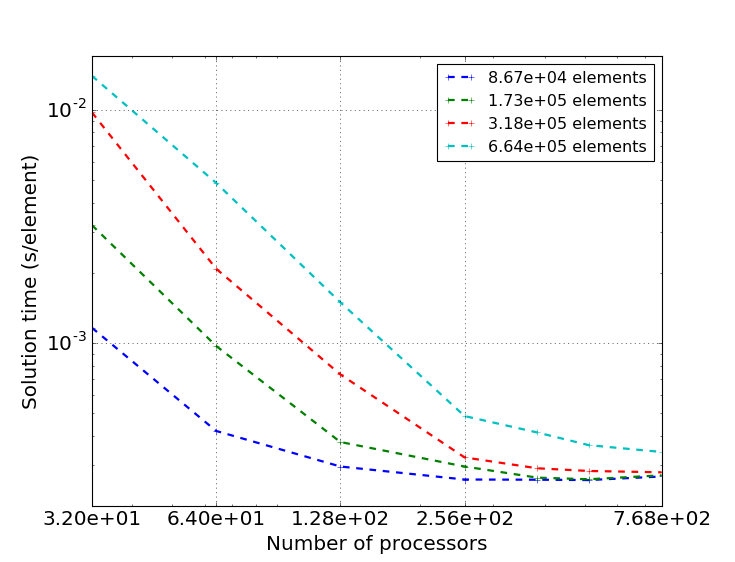
\includegraphics[width=1\linewidth]{extra-node_strong.png}
  \caption{Moltres extra-node strong scaling efficiency for various problem size, for $n_{nodes} \in [1,24]$.}
  \label{fig:extra_strong_scaling}
\end{figure}

For the weak scaling study, the part of the problem (workload) assigned
to each processor stays constant and additional elements are used to
solve a bigger problem which would not fit in memory on a single node.
Thus, the weak scaling measurement is justification for memory-bound
application such as multiphysics code. Linear weak scaling is achieved
when the execution time stays constant while the workload increasing
in direct proportion to the number of cores. We performed Moltres
weak-scaling tests on Blue Waters, keeping the workload constant at
581, 985, 1970 and 3940 elements per core. Fig.~\ref{fig:intra_weak} shows
Moltres weak scaling performance measured for $n_{cores} \in [1,32]$ within
one Blue Waters node and Fig.~\ref{fig:extra_weak} demonstrates performance
for $n_{cores} \in [32,128]$. As expected, the largest drop in performance
occurs when the number of cores increases from one to $\approx$ 8, which
corresponds to switching from no communication to a 2-D domain
decomposition. The further reduction in performance of only about 50\%
over a range of 32 cores is likely caused by increased communication
latency appearing from collective \gls{MPI} calls. In the extra-node case,
the performance drops by a factor of three, which is most likely due to poor node
selection by the Blue Waters job scheduler and significantly increased latency and
bandwidth costs.

\begin{figure}[htpb]
  \centering
  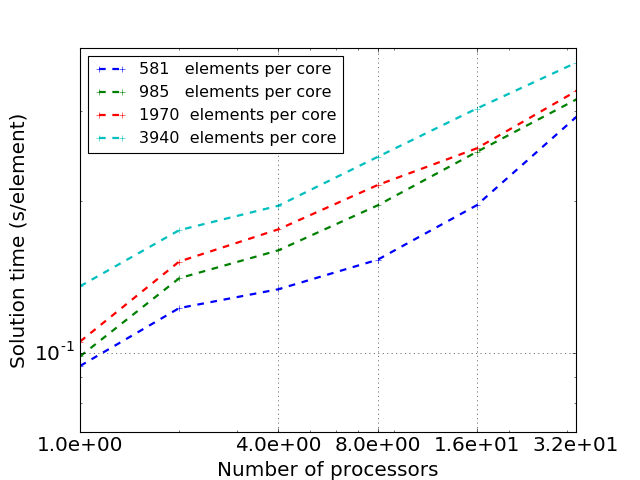
\includegraphics[width=\linewidth]{intra-node_weak.png}
  \caption{Weak scaling performance of Moltres on Blue Waters, in seconds per element vs. number of processors, for a constant number of elements
        per processor, and $n_{cores}\in[1,32]$.}
  \label{fig:intra_weak}
\end{figure}

\begin{figure}[htpb]
  \centering
  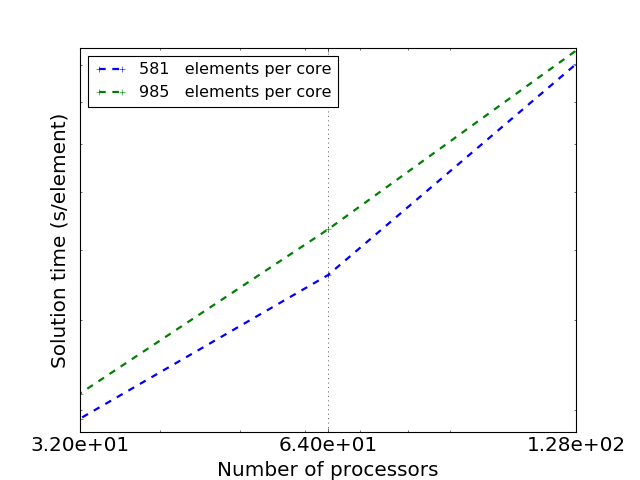
\includegraphics[width=\linewidth]{extra-node_weak.png}
  \caption{Weak scaling performance of Moltres on Blue Waters, in seconds per element vs. number of processors, for a constant number of elements
        per processor, for and $n_{cores}\in[32,128]$.}
  \label{fig:extra_weak}
\end{figure}

Moltres scalability study results clearly indicate that parallelization
using LibMesh's automatic domain decomposition is good, but not perfectly
efficient. This scaling performance is satisfactory for \gls{MSR} simulations
approached thus far and improved parallel performance would require further optimization
within LibMesh.  Moreover, Moltres is memory-bound and therefore very sensitive to host memory and memory
bandwidth. Consequently, if improved performance is needed, one could consider a transition from CPUs
computing to GPU-accelerated computing because GPUs operate on the fly with
global memory, avoiding CPU cache storage issues. Another way
to improve parallel performance is to force the solver to use
``older'' information from previous iterations. However, this has been shown to
slow convergence in terms of iterations and increased workload
\cite{satish_balay_petsc_2015}.

\begin{figure}[htpb!]
  \centering
  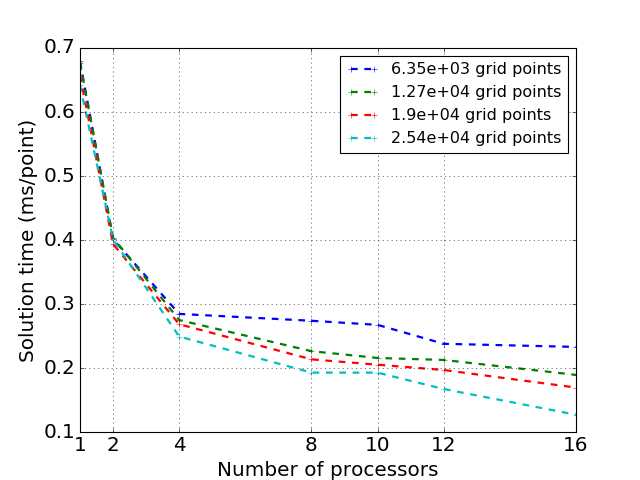
\includegraphics[width=\linewidth]{lapl_strong_time.png}
  \caption{Strong scaling execution time per grid point for 2-D Poisson's equation solver.}
  \label{fig:lapl_strong_time}
\end{figure}
\FloatBarrier

\subsection{Parralel preconditioned Conjugate Gradient solver scaling study}

As discussed earlier, to evaluate parallelization efficiency of Moltres multiphysics code simple solver was developed based on
preconditioned Conjugate Gradient (CG) iterative method. Classic Jacobi preconditioner was used to accelerate convergence. 

\begin{figure}[htpb!]
  \centering
  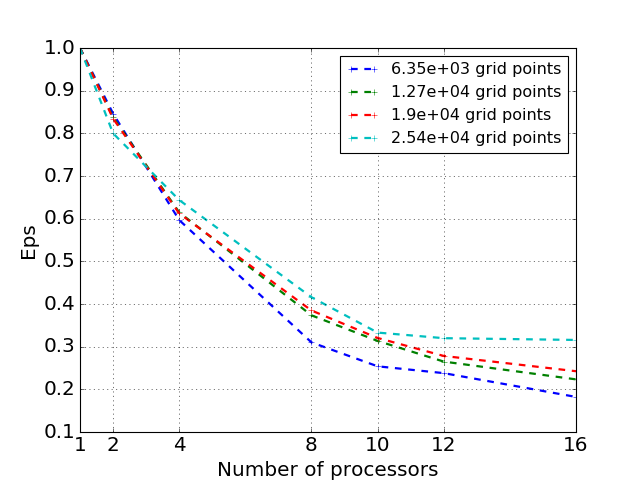
\includegraphics[width=\linewidth]{lapl_strong_eff.png}
  \caption{Strong scaling parallel efficiency for 2-D Poisson's equation solver.}
  \label{fig:lapl_strong_eff}
\end{figure}
\FloatBarrier

We conducted strong and weak scaling studies to characterize parallel performance for the iterative solver. Fig.~\ref{fig:lapl_strong_time} shows the simulation speed in milliseconds per grid point vs. the number of cores on 1 node (maximum 16 cores). Up to 4 cores, it shows good speedup, while beyond 4 cores, scaling demonstrates asymptotic dependence on the number of processors due to increasing
communication costs. From fig.~\ref{fig:lapl_strong_eff} could be observed that the parallel efficiency for the strong scaling study is decreasing dramatically for the case from 1 to 0.2 for the smallest input (6348 points) and in the range from 1 to 0.33 for the largest input (25'392 points). Such a horrible parallel efficiency most likely happens due to a fixed number of iteration (>10000) instead of using Jacobi or Gauss-Seidel methods and will be fixed in a future version of the solver.

Fig.~\ref{fig:lapl_weak_time},\ref{fig:lapl_strong_eff} demonstrates results of weak scaling study when input size was fixed (1587 points per processor). Linear weak scaling is achieved when the execution time stays constant while the workload increasing
in direct proportion to the number of cores. The largest drop in performance occurs when the number of cores increases from one to $\approx$ 8, which corresponds to switching from no communication to a 2-D domain decomposition. The further reduction in performance is only about 10\% over a range of 16 cores is likely caused by increased communication latency appearing from collective \gls{MPI} calls. Similarly to strong scaling case, weak scaling parallel efficiency drops significantly from 1.0 to 0.3 most likely because the very small input was selected. For the few orders of magnitude larger workload efficiency of weak scaling expected to be much better. Moreover, Jacobi or Gauss-Seidel convergence checker will be implemented as discussed earlier for strong scaling study.

\begin{figure}[htp!]
  \centering
  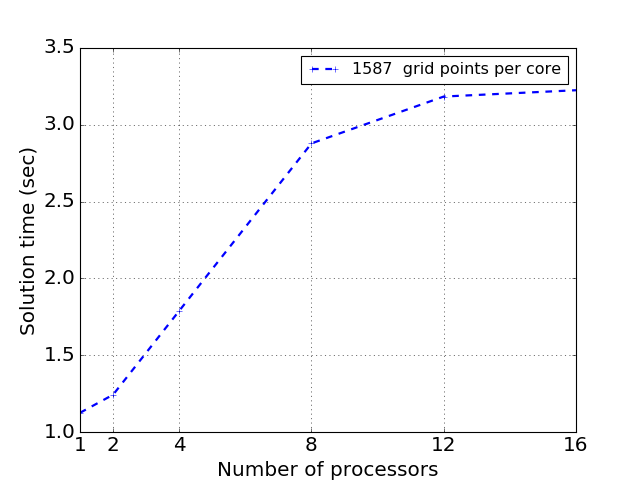
\includegraphics[width=\linewidth]{lapl_weak_time.png}
  \caption{Weak scaling execution time  for 2-D Poisson's equation solver.}
  \label{fig:lapl_weak_time}
\end{figure}
\FloatBarrier

\begin{figure}[htpb!]
  \centering
  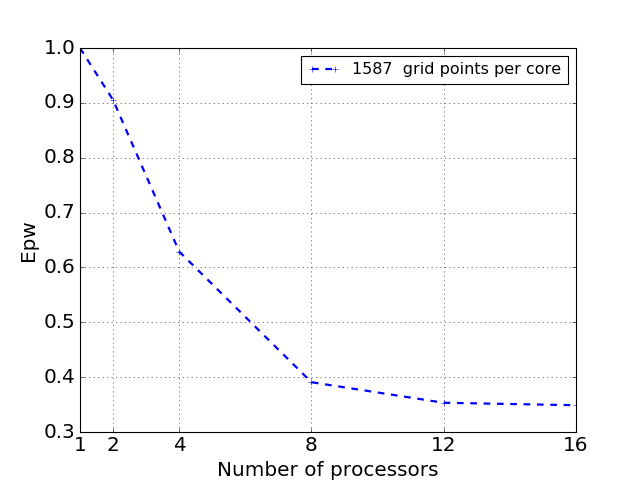
\includegraphics[width=\linewidth]{lapl_weak_eff.png}
  \caption{Weak scaling parallel efficiency for 2-D Poisson's equation solver.}
  \label{fig:lapl_weak_eff}
\end{figure}

\section{Future work}
\begin{itemize}
	\item Detail theoretical computational cost analysis will be performed to find sources of overhead.
	\vspace{-0.6em}
	\item Work underway to coupled multigroup diffusion and discontinuous Galerkin precursor transport to Navier-Stokes modules.
	\vspace{-0.6em}
	\item Effects of salt/graphite temperature change cross terms yet to be quantified.
	\vspace{-0.6em}
	\item Parallelization optimization tweaking parameters of preconditioners and solvers in PETSc (i.e. ILU parameters).
	\vspace{-1.6em}
	\item Precoursors decay heat implementation (expected ~8\% of total power).
	\vspace{-0.6em}
	\item Natural convection implementation using the Boussinesq approximation. 
	\vspace{-0.6em}
	\item Transition from CPUs computing to GPU-accelerated computing to avoid CPU cache storage issues.
	\vspace{-0.6em}
\end{itemize}

%%%%%%%%%%%%%%%%%%%%%%%%%%%%%%%%%%%%%%%%%%%%%%%%%%%%%%%%%%%%%%%%%%%%%%%%%%%%%%%%
\bibliographystyle{ans}
\bibliography{bibliography}
\end{document}

